\documentclass{article}

\usepackage{fullpage,latexsym,picinpar,amsmath,amsfonts}

\usepackage{graphicx}

           

%%%%%%%%%%%%%%%%%%%%%%%%%%%%%%%%%%%%%%%%%%%%%%%%%%%%%%%%%%%%%%%%%%%%%%%%%%%%%%%%%%%
%%%%%%%%%%%  LETTERS 
%%%%%%%%%%%%%%%%%%%%%%%%%%%%%%%%%%%%%%%%%%%%%%%%%%%%%%%%%%%%%%%%%%%%%%%%%%%%%%%%%%%

\newcommand{\barx}{{\bar x}}
\newcommand{\bary}{{\bar y}}
\newcommand{\barz}{{\bar z}}
\newcommand{\bart}{{\bar t}}

\newcommand{\bfP}{{\bf{P}}}

%%%%%%%%%%%%%%%%%%%%%%%%%%%%%%%%%%%%%%%%%%%%%%%%%%%%%%%%%%%%%%%%%%%%%%%%%%%%%%%%%%%
%%%%%%%%%%%%%%%%%%%%%%%%%%%%%%%%%%%%%%%%%%%%%%%%%%%%%%%%%%%%%%%%%%%%%%%%%%%%%%%%%%%
                                                                                
\newcommand{\parend}[1]{{\left( #1  \right) }}
\newcommand{\spparend}[1]{{\left(\, #1  \,\right) }}
\newcommand{\angled}[1]{{\left\langle #1  \right\rangle }}
\newcommand{\brackd}[1]{{\left[ #1  \right] }}
\newcommand{\spbrackd}[1]{{\left[\, #1  \,\right] }}
\newcommand{\braced}[1]{{\left\{ #1  \right\} }}
\newcommand{\leftbraced}[1]{{\left\{ #1  \right. }}
\newcommand{\floor}[1]{{\left\lfloor #1\right\rfloor}}
\newcommand{\ceiling}[1]{{\left\lceil #1\right\rceil}}
\newcommand{\barred}[1]{{\left|#1\right|}}
\newcommand{\doublebarred}[1]{{\left|\left|#1\right|\right|}}
\newcommand{\spaced}[1]{{\, #1\, }}
\newcommand{\suchthat}{{\spaced{|}}}
\newcommand{\numof}{{\sharp}}
\newcommand{\assign}{{\,\leftarrow\,}}
\newcommand{\myaccept}{{\mbox{\tiny accept}}}
\newcommand{\myreject}{{\mbox{\tiny reject}}}
\newcommand{\blanksymbol}{{\sqcup}}
                                                                                                                         
\newcommand{\veps}{{\varepsilon}}
\newcommand{\Sigmastar}{{\Sigma^\ast}}
                           
\newcommand{\half}{\mbox{$\frac{1}{2}$}}    
\newcommand{\threehalfs}{\mbox{$\frac{3}{2}$}}   
\newcommand{\domino}[2]{\left[\frac{#1}{#2}\right]}  

%%%%%%%%%%%% complexity classes

\newcommand{\PP}{\mathbb{P}}
\newcommand{\NP}{\mathbb{NP}}
\newcommand{\PSPACE}{\mathbb{PSPACE}}
\newcommand{\coNP}{\textrm{co}\mathbb{NP}}
\newcommand{\DLOG}{\mathbb{L}}
\newcommand{\NLOG}{\mathbb{NL}}
\newcommand{\NL}{\mathbb{NL}}

%%%%%%%%%%% decision problems

\newcommand{\PCP}{\sc{PCP}}
\newcommand{\Path}{\sc{Path}}
\newcommand{\GenGeo}{\sc{Generalized Geography}}

\newcommand{\malytm}{{\mbox{\tiny TM}}}
\newcommand{\malycfg}{{\mbox{\tiny CFG}}}
\newcommand{\Atm}{\mbox{\rm A}_\malytm}
\newcommand{\complAtm}{{\overline{\mbox{\rm A}}}_\malytm}
\newcommand{\AllCFG}{{\mbox{\sc All}}_\malycfg}
\newcommand{\complAllCFG}{{\overline{\mbox{\sc All}}}_\malycfg}
\newcommand{\complL}{{\bar L}}
\newcommand{\TQBF}{\mbox{\sc TQBF}}
\newcommand{\SAT}{\mbox{\sc SAT}}

%%%%%%%%%%%%%%%%%%%%%%%%%%%%%%%%%%%%%%%%%%%%%%%%%%%%%%%%%%%%%%%%%%%%%%%%%%%%%%%%%%%
%%%%%%%%%%%%%%% for homeworks
%%%%%%%%%%%%%%%%%%%%%%%%%%%%%%%%%%%%%%%%%%%%%%%%%%%%%%%%%%%%%%%%%%%%%%%%%%%%%%%%%%%

\newcommand{\student}[2]{%
{\noindent\Large{ \emph{#1} SID {#2} } \hfill} \vskip 0.1in}

\newcommand{\assignment}[1]{\medskip\centerline{\large\bf CS 111 ASSIGNMENT {#1}}}

\newcommand{\duedate}[1]{{\centerline{due {#1}\medskip}}}     

\newcounter{problemnumber}                                                                                 

\newenvironment{problem}{{\vskip 0.1in \noindent
              \bf Problem~\addtocounter{problemnumber}{1}\arabic{problemnumber}:}}{}

\newcounter{solutionnumber}

\newenvironment{solution}{{\vskip 0.1in \noindent
             \bf Solution~\addtocounter{solutionnumber}{1}\arabic{solutionnumber}:}}
				{\ \newline\smallskip\lineacross\smallskip}

\newcommand{\lineacross}{\noindent\mbox{}\hrulefill\mbox{}}

\newcommand{\decproblem}[3]{%
\medskip
\noindent
\begin{list}{\hfill}{\setlength{\labelsep}{0in}
                       \setlength{\topsep}{0in}
                       \setlength{\partopsep}{0in}
                       \setlength{\leftmargin}{0in}
                       \setlength{\listparindent}{0in}
                       \setlength{\labelwidth}{0.5in}
                       \setlength{\itemindent}{0in}
                       \setlength{\itemsep}{0in}
                     }
\item{{{\sc{#1}}:}}
                \begin{list}{\hfill}{\setlength{\labelsep}{0.1in}
                       \setlength{\topsep}{0in}
                       \setlength{\partopsep}{0in}
                       \setlength{\leftmargin}{0.5in}
                       \setlength{\labelwidth}{0.5in}
                       \setlength{\listparindent}{0in}
                       \setlength{\itemindent}{0in}
                       \setlength{\itemsep}{0in}
                       }
                \item{{\em Instance:\ }}{#2}
                \item{{\em Query:\ }}{#3}
                \end{list}
\end{list}
\medskip
}

%%%%%%%%%%%%%%%%%%%%%%%%%%%%%%%%%%%%%%%%%%%%%%%%%%%%%%%%%%%%%%%%%%%%%%%%%%%%%%%%%%%
%%%%%%%%%%%%% for quizzes
%%%%%%%%%%%%%%%%%%%%%%%%%%%%%%%%%%%%%%%%%%%%%%%%%%%%%%%%%%%%%%%%%%%%%%%%%%%%%%%%%%%

\newcommand{\quizheader}{ {\large NAME: \hskip 3in SID:\hfill}
                                \newline\lineacross \medskip }


%%%%%%%%%%%%%%%%%%%%%%%%%%%%%%%%%%%%%%%%%%%%%%%%%%%%%%%%%%%%%%%%%%%%%%%%%%%%%%%%%%%
%%%%%%%%%%%%% for final
%%%%%%%%%%%%%%%%%%%%%%%%%%%%%%%%%%%%%%%%%%%%%%%%%%%%%%%%%%%%%%%%%%%%%%%%%%%%%%%%%%%

\newcommand{\namespace}{\noindent{\Large NAME: \hfill SID:\hskip 1.5in\ }\\\medskip\noindent\mbox{}\hrulefill\mbox{}}



\begin{document}

\noindent
\emph{\large Alejandro Sherman} \large SID 862062898

\vskip 0.2in

\centerline{\large \bf CS/MATH111 RSA EXTRA CREDIT ASSIGNMENT}
\centerline{due Tuesday, October 29}

\vskip 0.1in


\vskip 0.2in
\vskip 0.2in



\begin{solution}
Solution is in c++ code:\\
The user is prompted for a public key - \\
Valid public keys tested($e$ , n):\\
23 55, 13 77, 7 143, 5 91, 7 95, 11 51, 9 33\\
The user is prompted to enter either e or d to encrypt or decrypt a message.\\
If encrypt is chosen, the message in the file "Encrypt.txt" is encrypted and the coded message is written to the file "EncryptOutput.txt".\\
If decrypt is chosen, the encoded message in the file "Decrypt.txt" is decrypted and the decoded message is written to the file "DecryptOutput.txt".\\
Encrypting and decrypting is according the the schema used previously, (A is 2, B is 3, ..., Z is 27, and space is 28).\\
The code was tested using four different quotes:\\
"EVERYTHING SHOULD BE MADE AS SIMPLE AS POSSIBLE BUT NOT SIMPLER"\\
"THE GREATEST GLORY IN LIVING LIES NOT IN NEVER FALLING BUT IN RISING EVERY TIME WE FALL"\\
"DO NOT GO WHERE THE PATH MAY LEAD GO INSTEAD WHERE THERE IS NO PATH AND LEAVE A TRAIL"\\
"YOU KNOW YOU ARE ON THE ROAD TO SUCCESS IF YOU WOULD DO YOUR JOB AND NOT BE PAID FOR IT"\\
See code below:\\
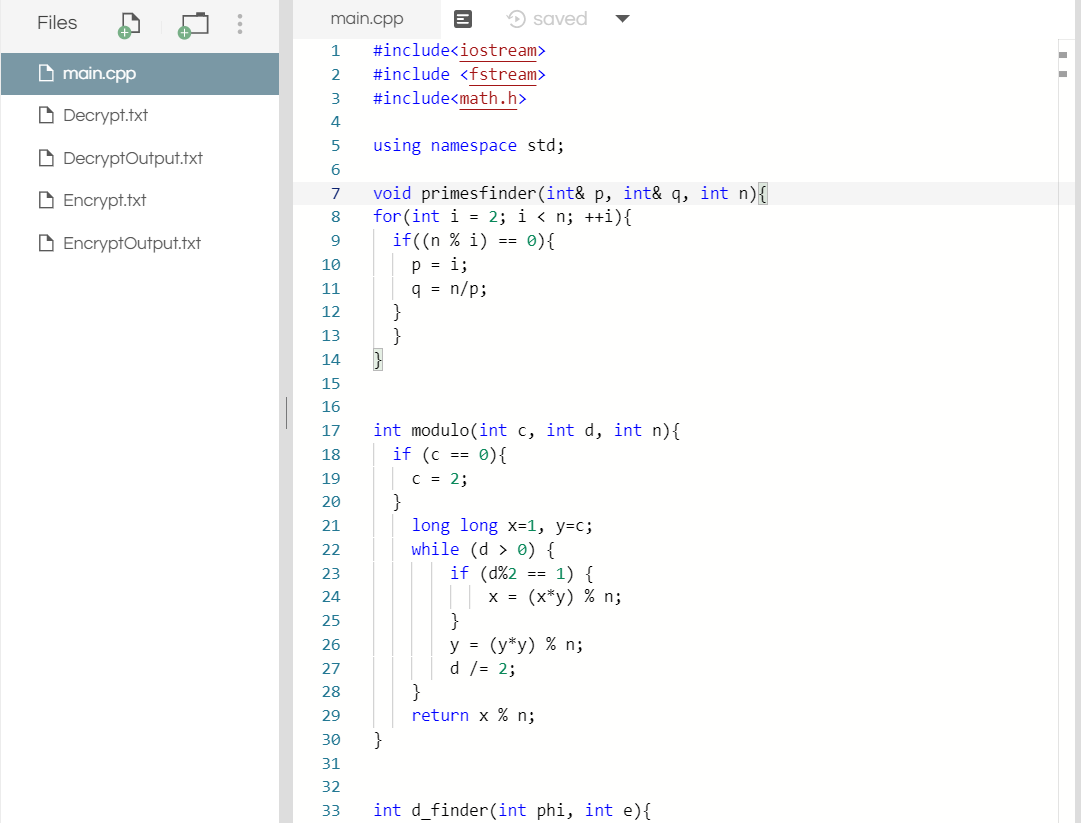
\includegraphics[width=16cm, height=16cm]{1a.png}\\
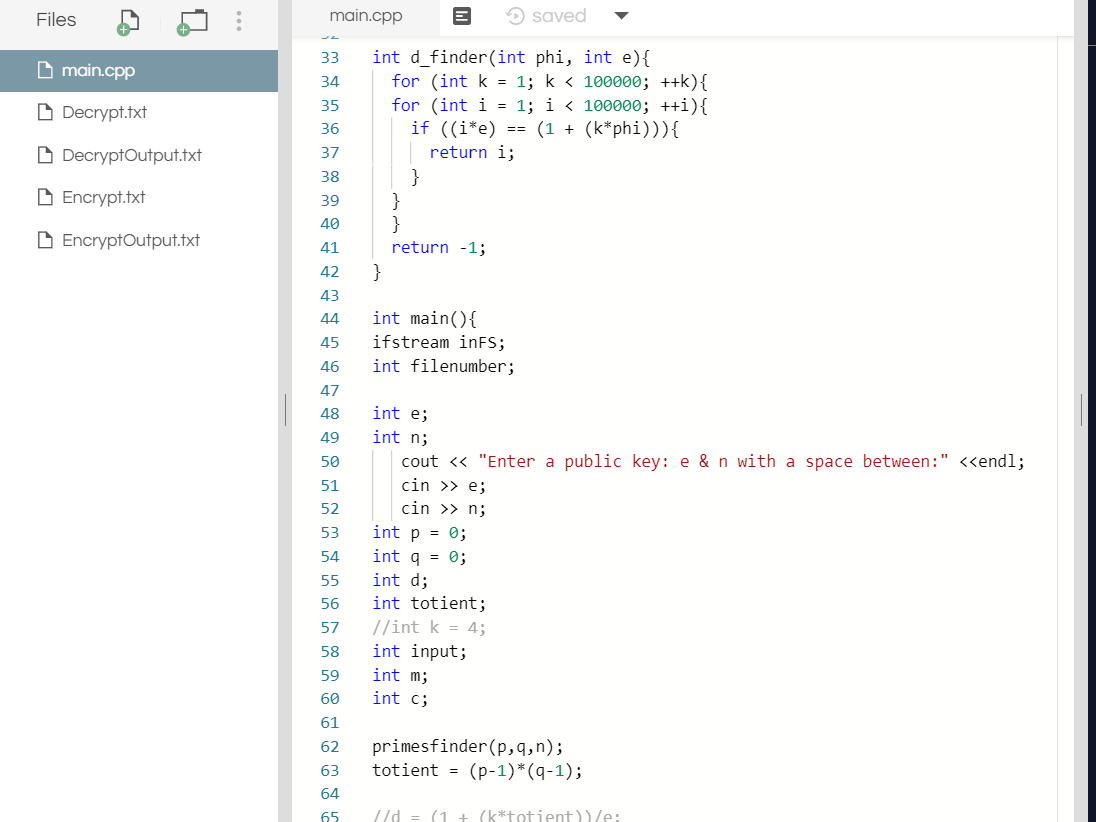
\includegraphics[width=16cm, height=16cm]{2a.png}\\
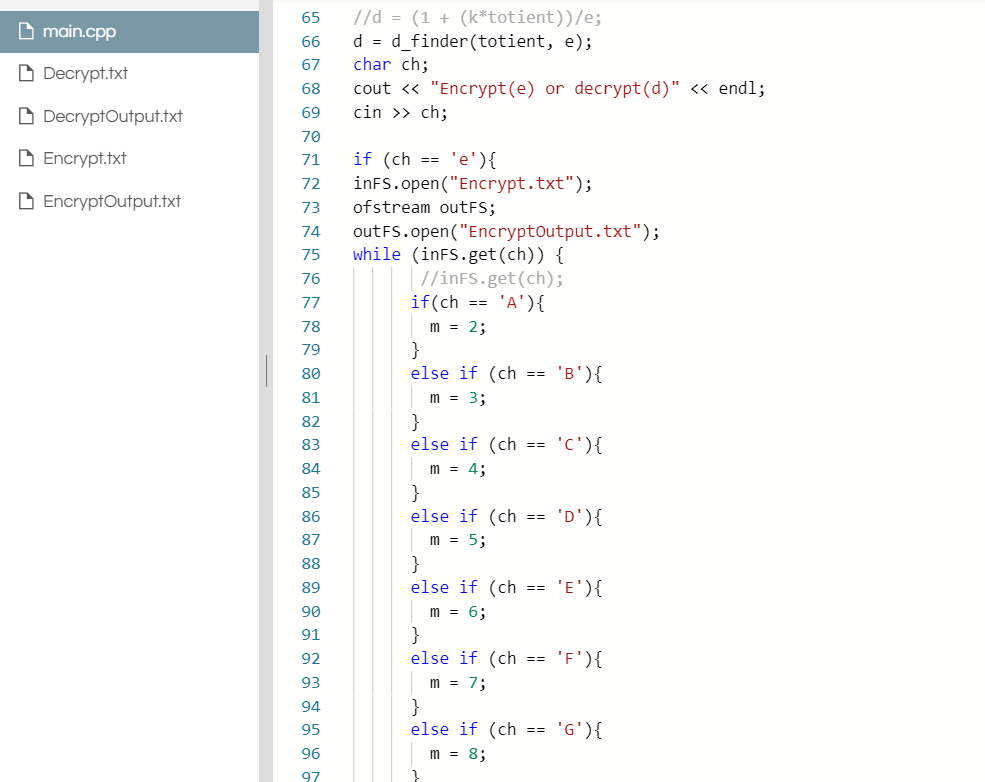
\includegraphics[width=16cm, height=16cm]{3a.png}\\
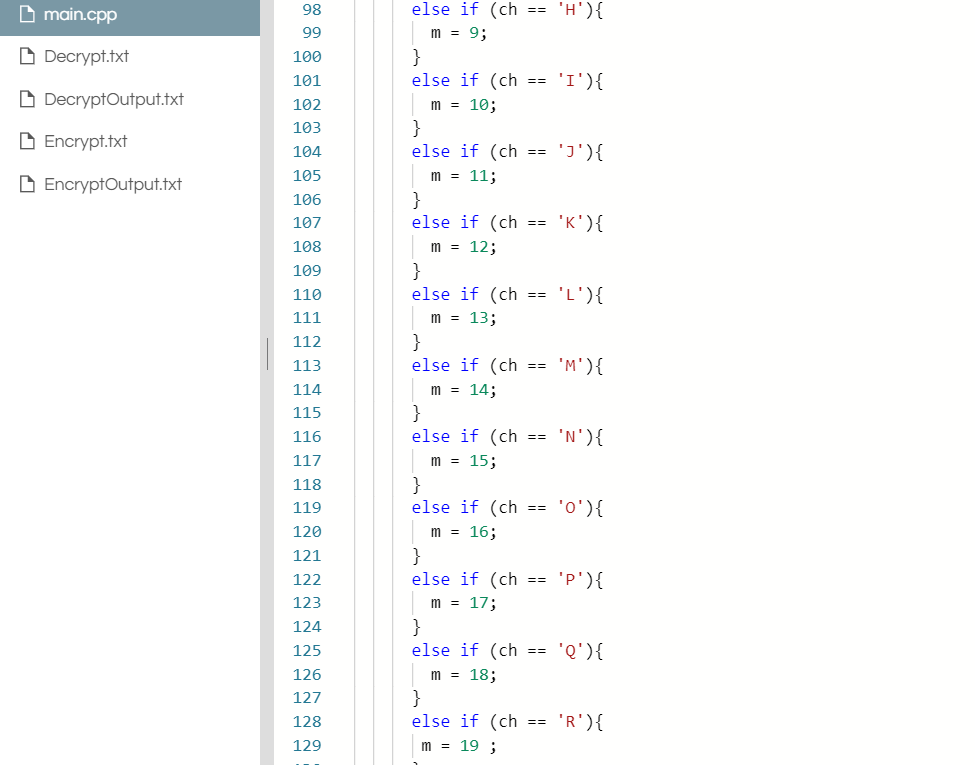
\includegraphics[width=16cm, height=16cm]{4a.png}\\
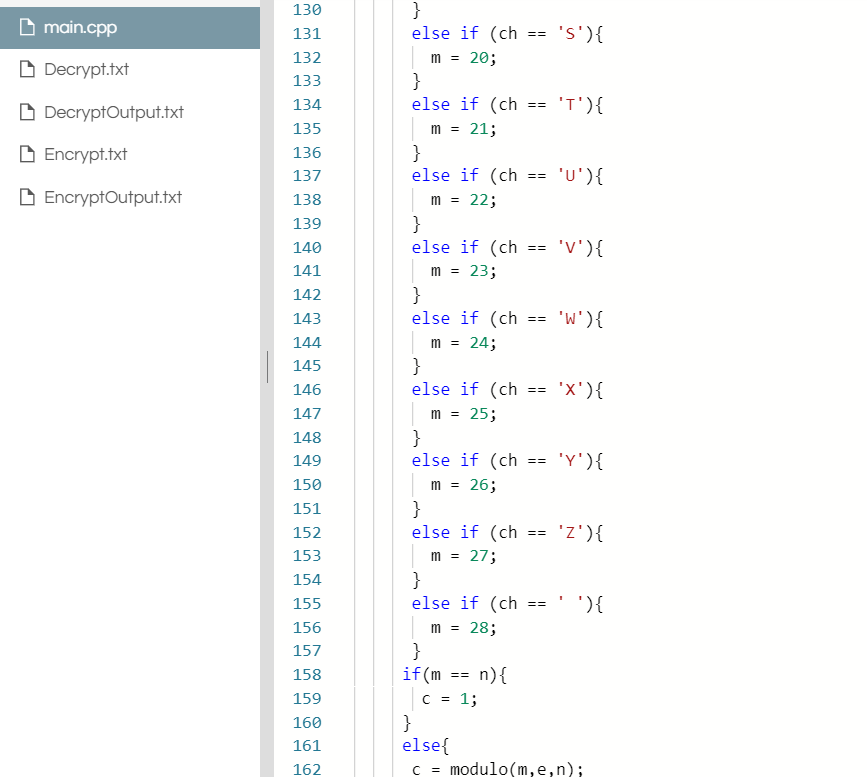
\includegraphics[width=16cm, height=16cm]{5a.png}\\
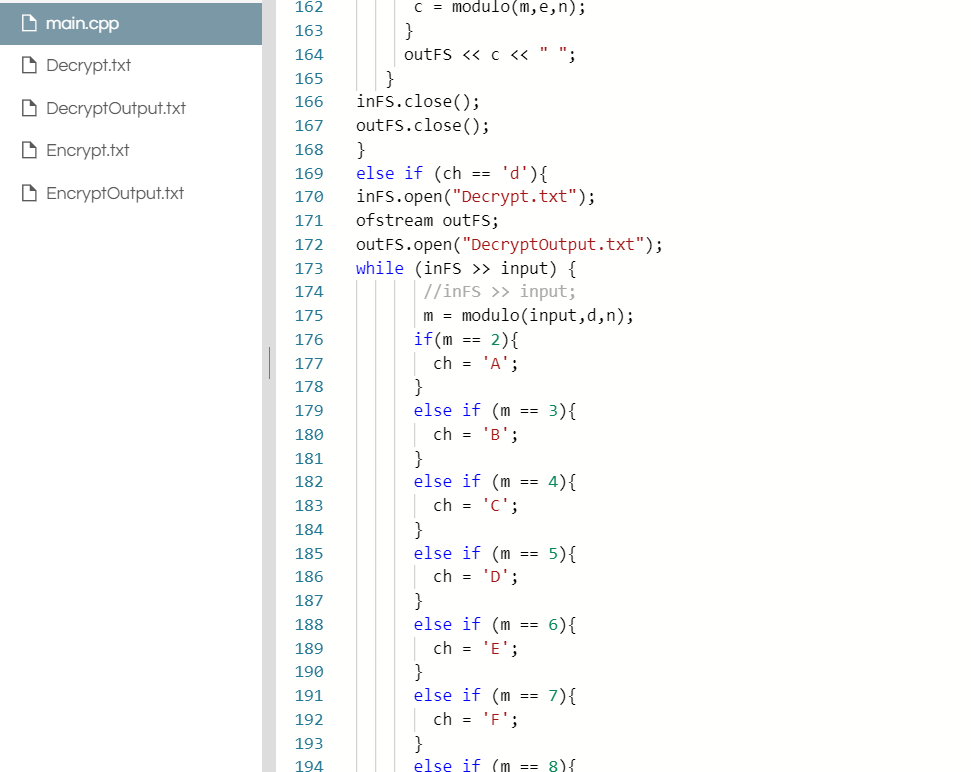
\includegraphics[width=16cm, height=16cm]{6a.png}\\
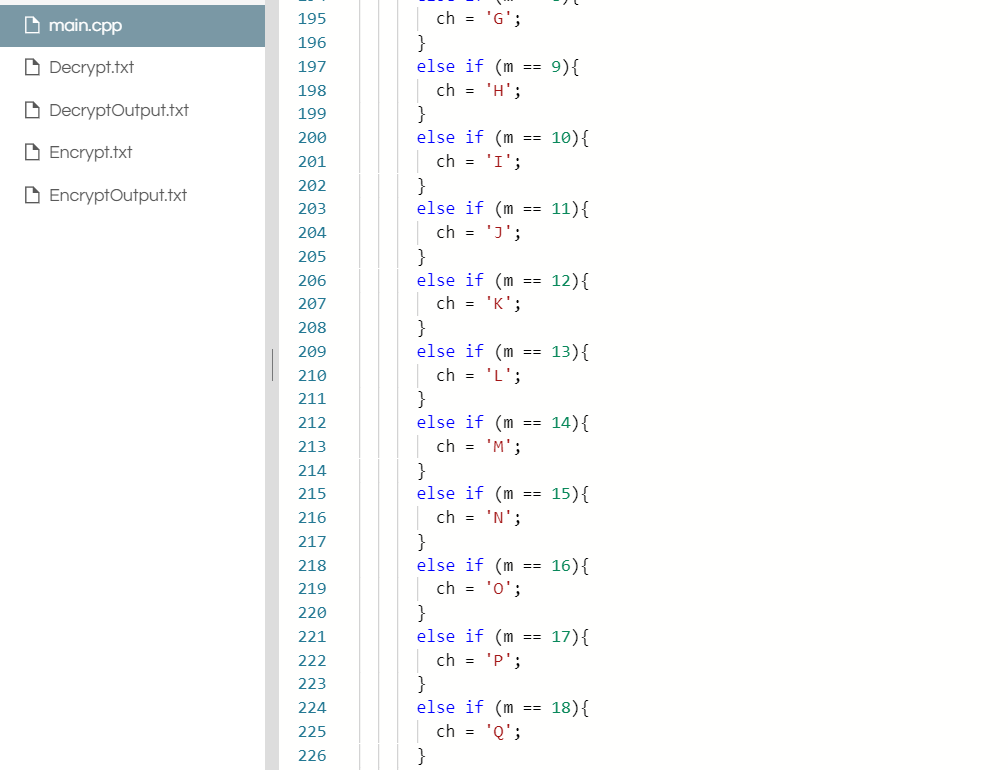
\includegraphics[width=16cm, height=16cm]{7a.png}\\
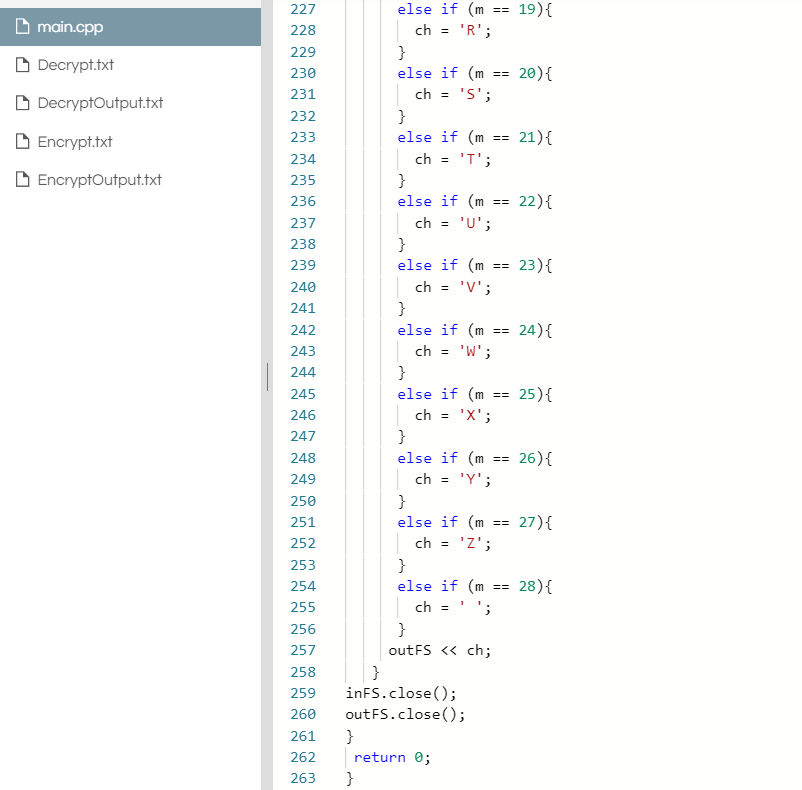
\includegraphics[width=16cm, height=16cm]{8a.png}\\
\vskip 0.5in
The following shows an example with the second listed quote, and the public key (11, 51).\\
Please see below:\\
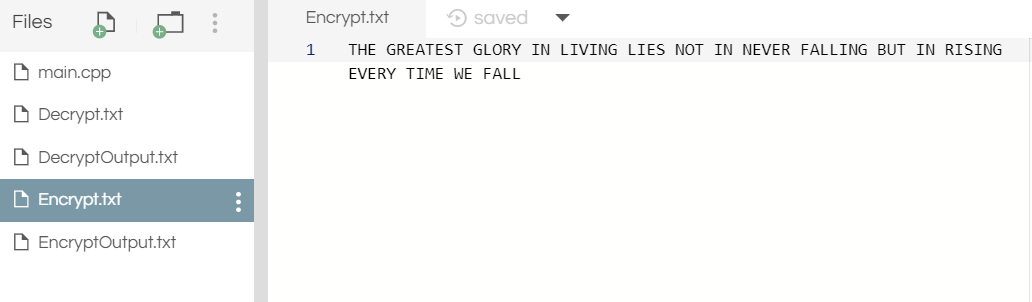
\includegraphics[width=16cm, height=6cm]{7.png}\\
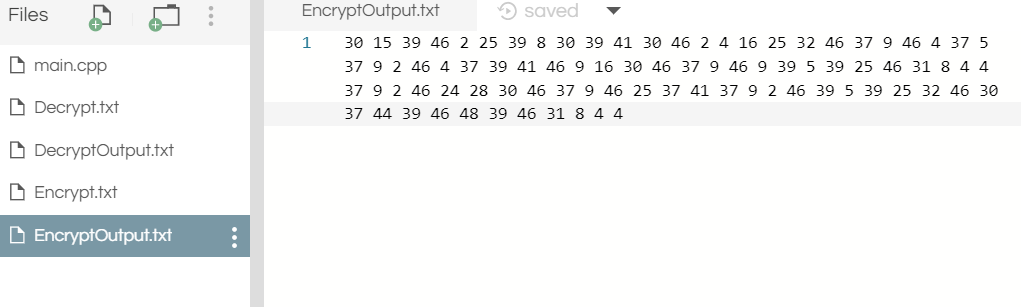
\includegraphics[width=16cm, height=6cm]{8.png}\\
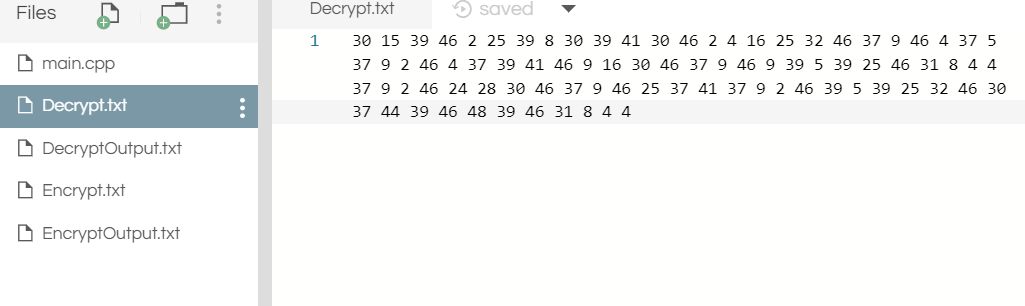
\includegraphics[width=16cm, height=6cm]{9.png}\\
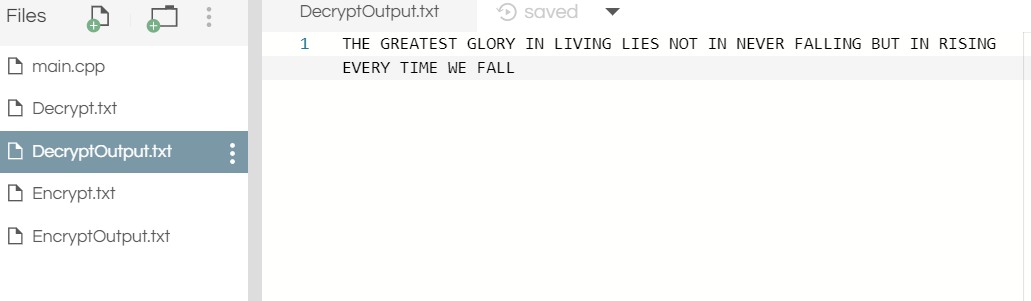
\includegraphics[width=16cm, height=6cm]{10.png}\\
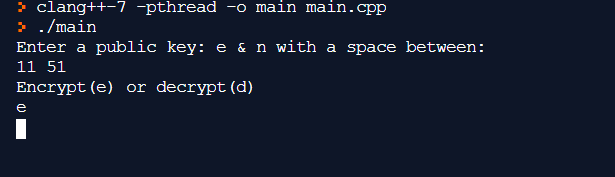
\includegraphics[width=16cm, height=4cm]{s.png}\\
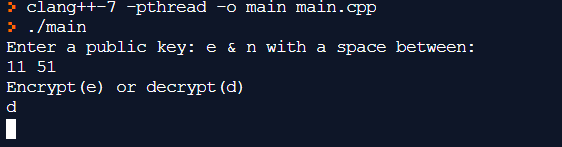
\includegraphics[width=16cm, height=4cm]{ss.png}\\
\end{solution}

\end{document}
